\documentclass[letterpaper,10pt]{article}

\usepackage{enumitem}
\usepackage{titling}
\usepackage{listings}
\usepackage{url}
\usepackage{hyperref}
\usepackage{setspace}
\usepackage{subfig}
\usepackage{sectsty}
\usepackage{pdfpages}
\usepackage{colortbl}
\usepackage{multirow}
\usepackage{multicol}
\usepackage{relsize}
\usepackage{amsmath}
\usepackage{wasysym}
\usepackage{fancyvrb}
\usepackage[yyyymmdd]{datetime}
\usepackage{amsmath,amssymb,amsthm,graphicx,xspace}
\usepackage[titlenotnumbered,noend,noline]{algorithm2e}
\usepackage[compact]{titlesec}
\usepackage{XCharter}
\usepackage[T1]{fontenc}
\usepackage[scaled]{beramono}
\usepackage[normalem]{ulem}
\usepackage{booktabs}
\usepackage{tikz}
\usetikzlibrary{arrows,automata,shapes,trees,matrix,chains,scopes,positioning,calc}
\tikzstyle{block} = [rectangle, draw, fill=blue!20,
text width=2.5em, text centered, rounded corners, minimum height=2em]
\tikzstyle{bw} = [rectangle, draw, fill=blue!20,
text width=4em, text centered, rounded corners, minimum height=2em]

\definecolor{namerow}{cmyk}{.40,.40,.40,.40}
\definecolor{namecol}{cmyk}{.40,.40,.40,.40}
\renewcommand{\dateseparator}{-}

\let\LaTeXtitle\title
\renewcommand{\title}[1]{\LaTeXtitle{\textsf{#1}}}

\lstset{basicstyle=\footnotesize\ttfamily,breaklines=true}

\newcommand{\handout}[5]{
	\noindent
	\begin{center}
		\framebox{
			\vbox{
				\hbox to 5.78in { {\bf ECE 350: Real-Time Operating Systems } \hfill #2 }
				\vspace{4mm}
				\hbox to 5.78in { {\Large \hfill #4  \hfill} }
				\vspace{2mm}
				\hbox to 5.78in { {\em #3 \hfill \today} }
			}
		}
	\end{center}
	\vspace*{4mm}
}

\newcommand{\lecture}[3]{\handout{#1}{#2}{#3}{Lecture#1}}
\newcommand{\tuple}[1]{\ensuremath{\left\langle #1 \right\rangle}\xspace}

\newcommand{\Rplus}{\protect\hspace{-.1em}\protect\raisebox{.35ex}{\smaller{\smaller\textbf{+}}}}
\newcommand{\Cpp}{\mbox{C\Rplus\Rplus}\xspace}


\addtolength{\oddsidemargin}{-1.000in}
\addtolength{\evensidemargin}{-0.500in}
\addtolength{\textwidth}{2.0in}
\addtolength{\topmargin}{-1.000in}
\addtolength{\textheight}{1.75in}
\addtolength{\parskip}{\baselineskip}
\setlength{\parindent}{0in}
\renewcommand{\baselinestretch}{1.5}
\newcommand{\term}{Spring 2023}
\newcommand{\termnumeric}{1235}

\singlespace


\begin{document}

\lecture{ 3 --- Sunrise to Sunset }{\term}{Jeff Zarnett}

\section*{Here When You Need Me}

We already learned about the lifecycle of a process, but the operating system itself has a lifetime as well. It needs to be started, it has a period where it executes, and will eventually shut down (for some reason or another). While it's running, it offers a number of services and a suite of functionality that is intended to make it easy and safe for user programs to execute.

\subsection*{Boot Up}
We will imagine the operating system is already installed on disk and not worry too much about systems without permanent storage (even though they did exist in the past). When you power on the computer the CPU execution at a predetermined location. This is in the BIOS (Basic Input-Output System), which is firmware, when it's an older computer. Newer computers use  UEFI (Unified Extensible Firmware Interface) that stores the boot information on disk rather than in the firmware itself. I don't want to get too bogged down in the details about how this works, but however it's implemented, it goes to the configured boot device (usually a hard drive)  and starts execution of the boot loader. 

What's a boot loader? It's a small piece of code whose purpose is to start up the operating system. This may be a multi-stage process involving loading a progressively-larger boot program from disk, but in the end, the goal is to load the kernel and begin its execution. The boot loader program may do other things, like verify the state of the machine and if the diagnostics are okay, proceed; it can also initialize things like the CPU registers, device controllers, wipe memory...~\cite{osc}.

The boot loader itself has at least some initialization code located in the first block of the hard drive that is the boot device. If the system has more than one drive, not all of them are necessarily configured for booting the system. Only if the first block of the drive contains this information can it be used for booting. The actual boot loader might be bigger. No matter how many steps it takes, eventually control is transferred to the kernel itself and then it's running.

\subsection*{What Can You Do For Me?}

Our previous experience with systems programming has taught us a lot about the services that the operating system has to offer. Some examples of things we already did:
\begin{multicols}{2}
\begin{itemize}
	\item Process and thread creation, termination
	\item Inter-process communication
	\item Concurrency control
	\item Memory allocation
\end{itemize}
\end{multicols}

The operating system does a lot more than this, and the visibility of that functionality varies. The OS must check permissions whenever you want to open a file, but you probably do not notice or think about it unless somehow permission is denied. There is scheduling, which we had to think about when it comes to concurrency and synchronization, but it was treated as external forces and nothing we could control. And then there are yet other things that the operating system does independently and we may or may not have any way of interacting with them, like the accounting and record keeping the system does.

A visual representation of that from~\cite{osc}:
\begin{center}
	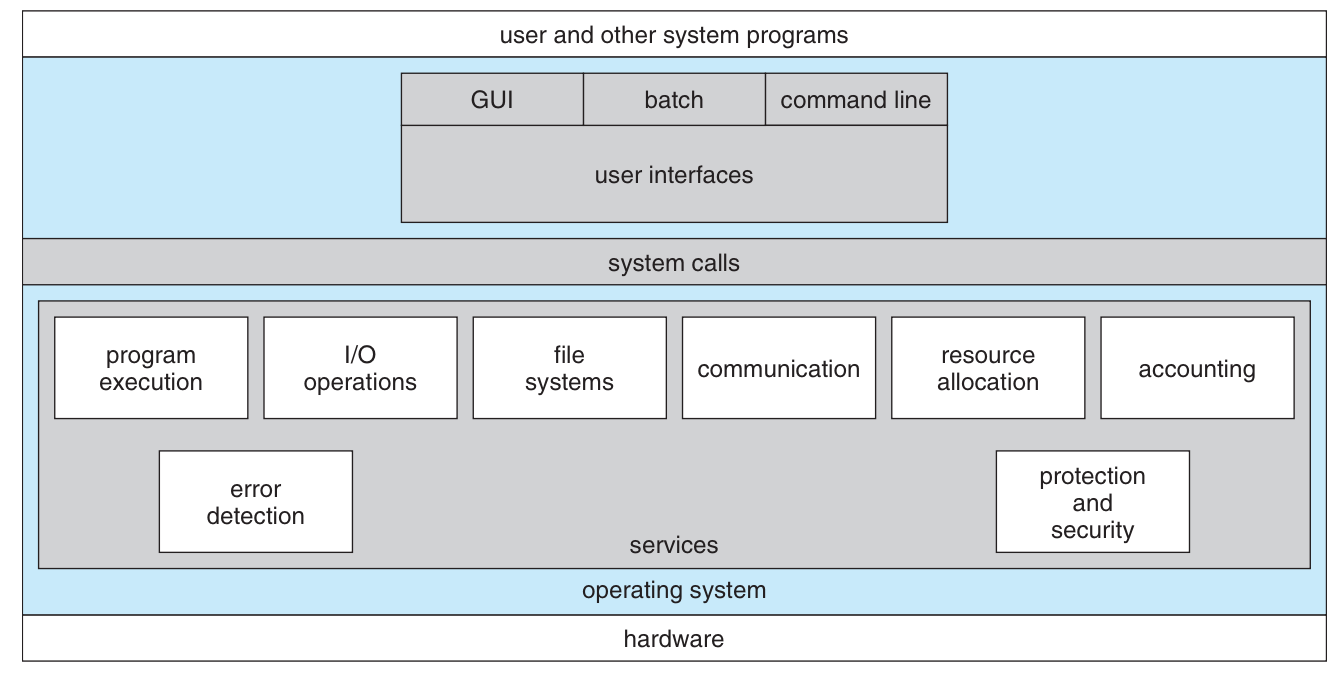
\includegraphics[width=0.75\textwidth]{images/os-structure.png}
\end{center}

At steady-state, the operating system runs whatever background tasks it needs to do, but the interesting things happen as the result of a user-level program asking for the OS to do something. And you know how that works...

\subsection*{System Calls: Remember, it's a Trap}

Previously, we covered this from the point of view of a user program that wants to activate the kernel. We said that it operates on interrupts and the interesting thing is the intentional use of the trap: this is how a user program gets the operating system's attention. When a user program is running, the operating system is not; we might even say it is ``sleeping''. If the program running needs the operating system to do something, it needs to wake up the OS: interrupt its sleep. When the trap occurs, the interrupt handler (part of the OS) is going to run to deal with the request.

Remember we saw the concept of user mode vs. supervisor mode instructions: some instructions are not available in user mode. Supervisor mode, also called kernel mode, allows all instructions and operations. Even something seemingly simple like reading from disk or writing to console output requires privileged instructions. These are common operations, but they involve the operating system every time.

Modern processors keep track of what mode they are in with the mode bit. This was not the case for some older processors and some current processors have more than two modes, but we will restrict ourselves to dual-mode operation with a mode bit. Thus we can see at a glance which mode the system is in. At boot up, the computer starts up in kernel mode as the operating system is started and loaded. User programs are always started in user mode. When a trap or interrupt occurs, and the operating system takes over, the mode bit is set to kernel mode; when it is finished the system goes back to user mode before the user program resumes~\cite{osc}.

Suppose a text editor wants to output data to a printer. Management of I/O devices like printers is the job of the OS, so to send the data, the text editor must ask the OS to step in, as in the diagram below:

\begin{center}
	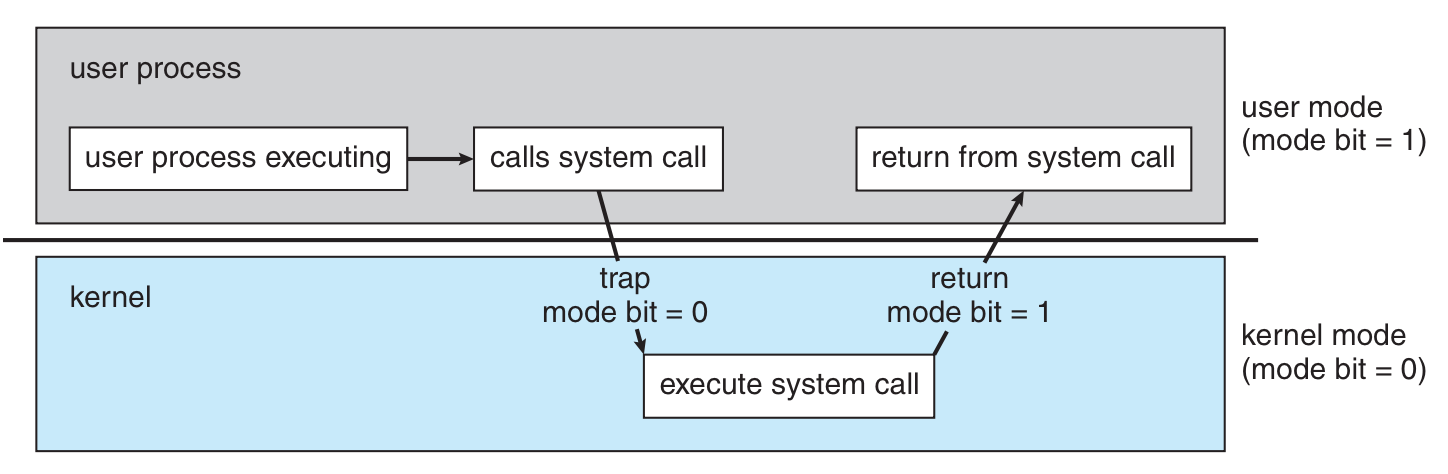
\includegraphics[width=0.75\textwidth]{images/trap.png}\\
	Transition from user to supervisor (kernel) mode~\cite{osc}.
\end{center}


So to print out the data, the program will prepare the data for printing. Then it calls the system call. You may think of this as being just like a normal function call, except it involves the operating system. This triggers the operating system (with a trap). The operating system responds and executes the system call and dispatches that data to the printer. When this job is done, operation goes back to user mode and the program returns from the system call.

\paragraph{Motivation for Dual Mode Operation.}

Why do we have user and supervisor modes, anyway? As Uncle Ben told Spiderman, ``with great power comes great responsibility''. Many of the reasons are the same as why we have user accounts and administrator accounts: we want to protect the system and its integrity against errant and malicious users.

An example: multiple programs might be trying to use the same I/O device at once. If Program~1 tries to read from disk, it will take time for that request to be serviced. During that time, if Program~2 wants to read from the same disk, the operating system will force Program~2 to wait its turn. Without the OS to enforce this, it would be up to the author(s) of Program~2 to check if the disk is currently in use and to wait patiently for it to become available. That may work if everybody plays nicely, but without someone to enforce the rules, sooner or later there will be a program that does something nasty, like cancel another program's read request and perform its read first.

This doesn't come for free, of course: there is a definite performance trade-off. Switching from user mode to kernel mode requires some instructions and some time. It would be faster if everything ran in kernel mode because we would spend no time switching. Despite this, the performance hit for the mode switch is judged worthwhile for the security and integrity benefits it provides.

\paragraph{Making it Happen}


\bibliographystyle{alphaurl}
\bibliography{350}


\end{document}